\documentclass[letterpaper, 10pt]{article}

% % % % % % % % % % % % % %
% Preamble
% % % % % % % % % % % % % %
 
%Get all the formatting details from preamble.tex
% % % % % % % % % % % % % %
% Package Imports
% % % % % % % % % % % % % %
%\usepackage[paperheight=28cm, paperwidth=22cm, includehead,
%nomarginpar, textwidth=18cm, headheight=20mm,footheight=20mm]{geometry}
\usepackage[letterpaper,textwidth=180mm,top=40mm,textheight=210mm]{geometry}
%\geometry{showframe=true}
\usepackage{graphicx}               % Required for inserting images
\usepackage{fancyhdr}               % Required for headers and footers
\usepackage{titling}                % Required to reformat the title
\usepackage{multicol}               % Required to use multiple columns in the doc
\usepackage[dvipsnames]{xcolor}     % Required to change the color of section headings
\usepackage{sectsty}                % Required to change the color of section headings
\usepackage[style=ieee]{biblatex}   % Required to make the bibliography
\usepackage[T1]{fontenc}            % Required to set the font
\usepackage{helvet}                 % Tells LaTeX to use helvetica font
\usepackage[hidelinks]{hyperref}               % Required to embed hyperlinks. 
\usepackage{tablefootnote}
\usepackage{svg}
    
\usepackage{lipsum}     % Lorem Ipsum generator, can be removed. 


% % % % % % % % % % % % % %
% Macros and Custom Commands
% % % % % % % % % % % % % %

%Update the title header. 
\renewcommand\maketitlehooka{%
  \setlength\parindent{0pt}%
  %\begin{minipage}{\textwidth}
    \begin{minipage}[b][.10\textheight][t]{\textwidth}
        \centering \small{\textbf{UNCLASSIFIED}}\\
    \begin{minipage}{.50\textwidth}
      
\includegraphics[width=\textwidth]{arlis}
    \end{minipage}%
    \begin{minipage}{.50\textwidth}
      \raggedleft
      \textbf{Technical Report}\par
      %\textbf{Summer 2023 Internship Program}\par
      %\textbf{Midprogram Status Report }\par
    \end{minipage}%
  \end{minipage}
  \par
  }

%Custom Comment Macros
\newcommand{\pinaforecomment}[4]{\colorbox{#1}{\textcolor{#4}{\parbox{.8\linewidth}{#2: #3}}}}
\newcommand{\osullikomment}[1]{\pinaforecomment{green}{Kent}{#1}{black}}
\newcommand{\nandirComment}[1]{\pinaforecomment{blue}{Nandini}{#1}{white}}
\newcommand{\vladComment}[1]{\pinaforecomment{orange}{Vlad}{#1}{black}}
\newcommand{\amirComment}[1]{\pinaforecomment{violet}{Amir}{#1}{white}}
\newcommand{\billComment}[1]{\pinaforecomment{Red}{Bill}{#1}{white}}


%Make header and footer hlines invisible
\renewcommand{\headrulewidth}{0pt} 
\renewcommand{\footrulewidth}{0pt}

%Left-Align the Abstract
\renewcommand*\abstractname{\flushleft{\textbf{Abstract} }}

%Make the color that is used in ARLIS branding
\definecolor{arlisRed}{HTML}{c33c35}

%Define the bibliogaphy
\bibliography{Bibliography/hive.bib}               %Source file for the bibliography, update if needed. Assumes in same directory, add full file path if not. 
\AtBeginBibliography{\footnotesize}   %adjust this size to \normal to match rest of doc if desired. 


% % % % % % % % % % % % % %
% Document Config
% % % % % % % % % % % % % %

%Tell LateX where to find images
\graphicspath{ {./Figures/} }

%Title Format
\setlength{\droptitle}{-100pt}
\pretitle{\begin{flushleft}\LARGE}
\posttitle{\par\end{flushleft}\vspace{-1em}}
\preauthor{\begin{flushleft}\large}
\postauthor{\par\end{flushleft}\vspace{-1.5em}}
\predate{\begin{flushleft}\large}
\postdate{\par\end{flushleft}\vspace{-2em}}

%Make the section and subsection headings red
\sectionfont{\color{arlisRed}}  % sets colour of sections
\subsectionfont{\color{arlisRed}}



\begin{document}
\pagestyle{empty}

%Make the title block
\title{\color{arlisRed}{
    \LARGE{Unlocking the Power of Hierarchical Identify Verify Exploit (HIVE): Revolutionizing Data Analysis and Efficiency }\\ 
    \large{Team MN}}}
\author{                                                            %Add as many authors as you like on new lines   
    \color{arlisRed}{
        Nandini Ramachandran, University of Maryland, nandinir@umd.edu}\\
        Morein Ibrahim, University of Maryland, morein04@terpmail.umd.edu \\
        Kent O'Sullivan, University of Maryland, osullik@umd.edu\\
    \small{\color{black}{                                           %Add as many POCs / mentors as you like on new lines
        \textbf{Sponsoring Agency:} DARPA\\
        \textbf{RISC Faculty Mentor 1:} William Regli, University of Maryland, regli@umd.edu \\
        \textbf{RISC Faculty Mentor 2:} Cliston Cole, Morgan State University, Cliston.cole@morgan.edu \\ 
    }} 
}

% % % % % % % % % % % % % %
% Headers and footers
% % % % % % % % % % % % % %
\pagestyle{fancy}
\fancyhead{}        %Flush the header and footer
\fancyfoot{}
%Header
\fancyhead[C]{\small{\textbf{SECURITY//LABELS//HERE}}\vspace{55pt}}
%Footer
\fancyfoot[C]{\thepage\\ DOD distribution statements go here. \\ © 2023 UMD/ARLIS. All Rights Reserved. Proprietary Information. \textbf{\\SECURITY//LABELS//HERE} }


% % % % % % % % % % % % % %
% Document Content
% % % % % % % % % % % % % %

\maketitle

\abstractname{}
\newline\par
\setlength{\parindent}{20pt}
Graph analytics has emerged as a critical tool for intelligence and security applications, enabling the analysis of complex relationships and patterns within interconnected data. The DARPA HIVE project aims to develop an advanced graph analytics processor that surpasses current technologies in terms of processing speed and power consumption. This research report presents the beginnings of a framework focused on evaluating the performance of fundamental graph processing algorithms such as community detection, subgraph matching, and knowledge graphs on CPU, GPU, and PiUMA architectures. The report emphasizes the importance of graph analysis in intelligence and security domains, outlines the methodology for evaluating performance using different algorithms and hardware configurations, discusses reference algorithm implementations, and highlights the progress of the study. The report aims to provide valuable insights into PiUMA's capabilities and contribute to advancements in graph processing technologies for intelligence and security applications.

\begin{multicols}{2}    
    \section{Project Goals}\label{section:goals}
    
    \billComment{Demo Comment}
    \clistonComment{Demo Comment}
    \moreinComment{Demo Comment}\\
    Team Minnesota's project sits within the Hierarchical Identify Verify Exploit (HIVE) program overseen by the Defense Advanced Research Project Agency (DARPA)\footnote{\href{https://www.darpa.mil/program/hierarchical-identify-verify-exploit}{https://www.darpa.mil/program/hierarchical-identify-verify-exploit}}. The ARLIS Statement of Work (SOW) identifies several goals for the project, discussed below. 
        \subsection{Overarching Project Goal}\label{section:projectGoal}
        The HIVE program seeks to develop an advanced graph processor capable of efficiently processing streaming graphs 1000x faster, while reducing power consumption. 
        Team Minnesota's role within the program is to develop a benchmarking suite to measure the progress of Intel's Programmable Integrated Unified Memory Architecture (PIUMA), and any other following efforts make towards the performance goals. 
        The benchmark suite must be specific to evaluating performance on problems specific to the intelligence and security domain.
        \subsection{Sub Goals}\label{section:subGoals}
        \begin{enumerate}
        \item Collect datasets that are representative of intelligence and security problems typically approached with graph analysis. 
        \item Source or develop suitable cross-architecture reference implementations of graph analysis algorithms commonly used by the intelligence and security community. 
        \item Construct an experimental framework that is able to report performance in terms of execution time, memory usage and power consumption.
        \item Benchmark PiUMA, a new architecture for high-performance graph processing utilizing against the provided projections 
        \end{enumerate}

        \subsection{Relevance to the Intelligence and Security Community} \label{section:relevance}
        
        \par{Many intelligence and security problems are fundamentally social problems. 
        Whether the goal is to determine the axis of advance for an enemy tank battalion, tracing transnational assassins\footnote{\href{https://www.bellingcat.com/resources/2020/12/14/navalny-fsb-methodology/}{https://www.bellingcat.com/resources/2020/12/14/navalny-fsb-methodology/}} identifying foreign intelligence officers\footnote{\href{https://www.wired.com/2007/07/in-italy-cia-agents-are-undone-by-their-cell-phones/}{https://www.wired.com/2007/07/in-italy-cia-agents-are-undone-by-their-cell-phones/}}, analyzing disinformation operations\footnote{\href{https://www.bellingcat.com/news/2019/09/03/twitter-analysis-identifying-a-pro-indonesian-propaganda-bot-network/}{https://www.bellingcat.com/news/2019/09/03/twitter-analysis-identifying-a-pro-indonesian-propaganda-bot-network/}} unmasking members of the GRU\footnote{\href{https://www.bellingcat.com/news/uk-and-europe/2020/10/22/russian-vehicle-registration-leak-reveals-additional-gru-hackers/}{https://www.bellingcat.com/news/uk-and-europe/2020/10/22/russian-vehicle-registration-leak-reveals-additional-gru-hackers/}} or trying to prevent human trafficking \cite{Szekely2015} we can frequently model these social problems as a collection of interactions between humans. 
        A powerful method of modeling human social behavior is through the use of a graph data structure.
        
        Formally, a Graph $G$ is a collection of Vertices (or nodes) $V$ and edges $E$ such that $G=\{V,E\}$.
        Consider the $PhoneRecords$ graph in figure \ref{fig:callRecords}. $PhoneRecords$ is made up of Vertices $PhoneNumbers$ and Edges $PhoneCalls$ that link $PhoneNumbers$ to each other.
        So, $PhoneRecords$ is therefore a graph that contains the set of all Phone Numbers and the calls between those numbers.}

        \begin{figure*}
            \centering
            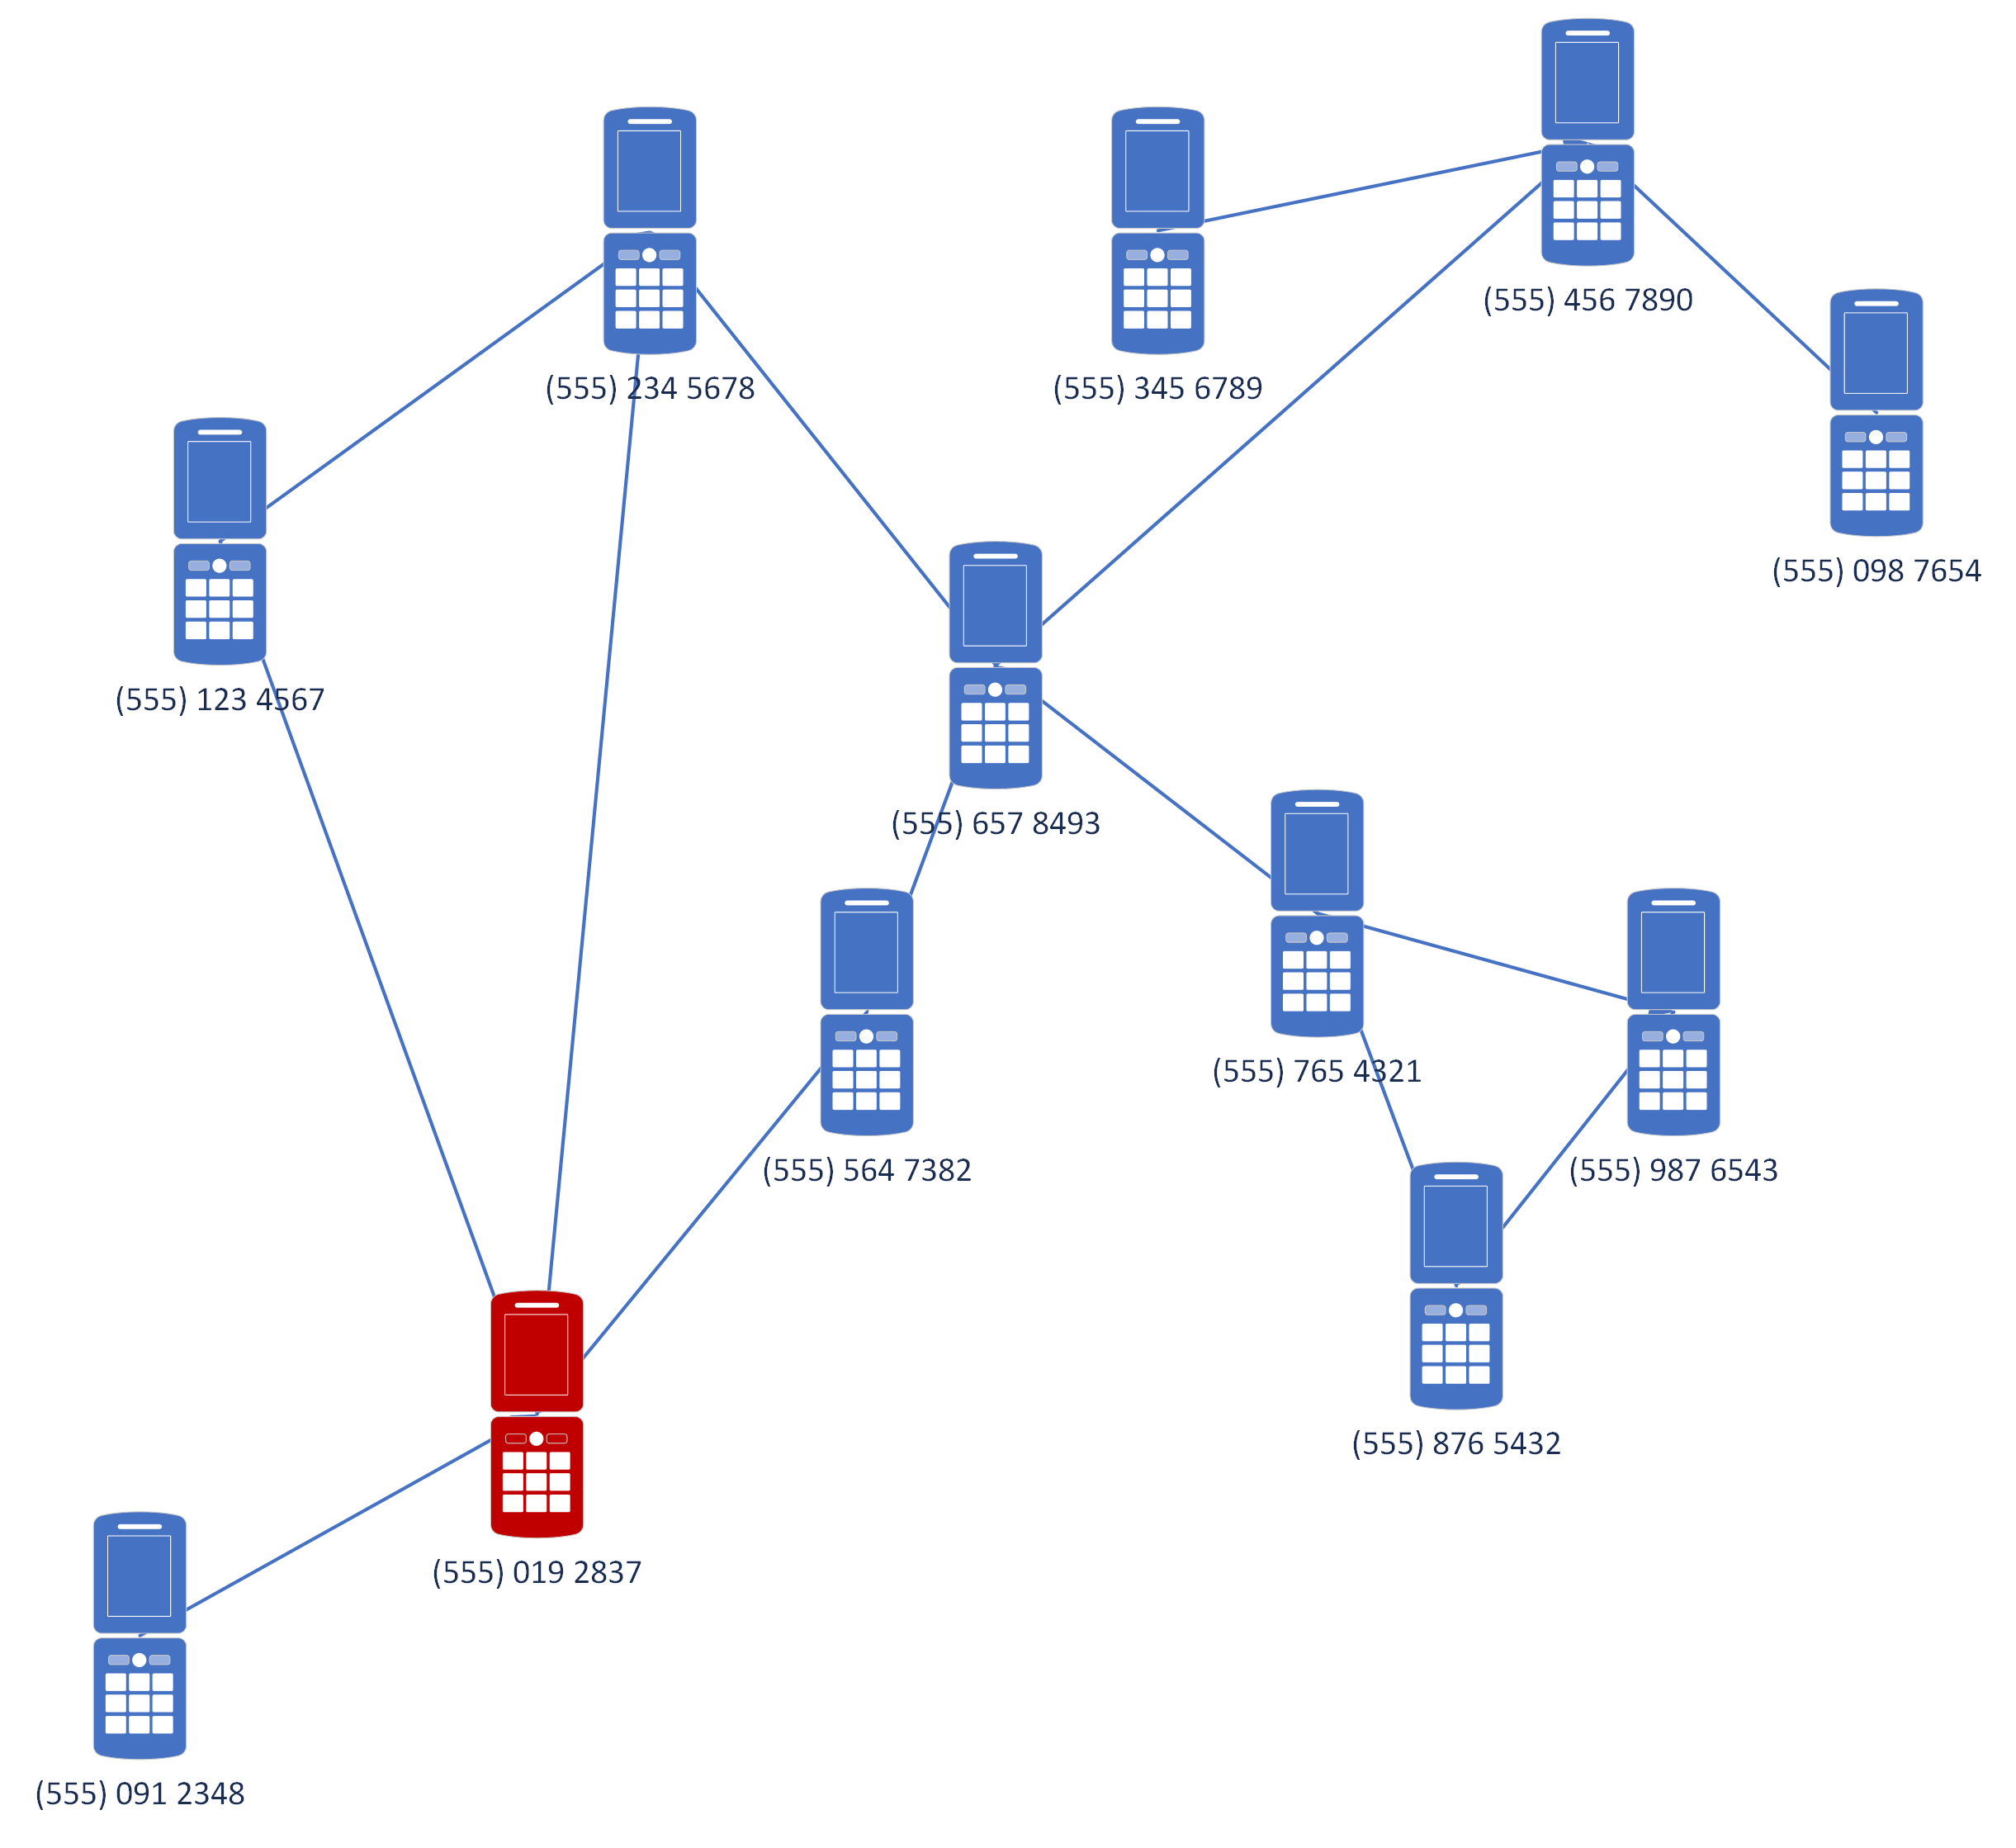
\includegraphics[width=\columnwidth]{Papers/ARLIS_MPR_MN/Figures/PhoneRecords.png}
            \caption{A Notional $CallRecords$ graph has phone numbers as the $Vertexes$ (or $nodes$) as phone numbers and the calls between those numbers as $Edges$. If the analyst knows the phone number of a person of interest (in red) they can use graph analytics to address intelligence requirements about the community the POI is involved with, where call patterns correlate with events or what possible multi-hop information flows could be.}
            \label{fig:callRecords}
        \end{figure*}
        
        Because of their powerful ability to model and query social interactions of intelligence interest, graphs are used extensively across the intelligence community to store and analyze important pieces of data. 

        Graph analysis is implemented through algorithms and techniques specifically designed to process and analyze graph data. 
        These algorithms traverse, explore, and extract insights from the interconnected nodes and edges of the graph. By identifying hidden patterns, facilitating decision-making, and enhancing situational awareness, graph analysis contributes to the overall security and defense efforts of a nation. 
        
        The problem motivating the HIVE program is that when these graphs get very large (say, if $PhoneCalls$ has all phone calls made by all numbers in the USA for the last 50 years) they become very slow to search and many problems quickly become intractable.
        Just as the advent of the GPU has breathed life into the neural network algorithms developed in the 80s and 90s by increasing the amount of available compute \cite{Dally2021}, HIVE expects that specialized hardware optimized for Graph Processing may make some of these 'intractable' problems solvable, and expand the toolkit available to the I\&S community. 
        
    \section{Background and Related Work}\label{section:background}
        \par{Towards determining whether the PiUMA system is a step towards the HIVE goal, we must consider our research in the context of prior work in graph workload benchmarking. 
        We summarize our preliminary review in terms of the available Datasets, Reference Algorithm implementations in Table \ref{table:graphAlgorithms}, supported metrics in table \ref{table:graphMetrics} and available System Architectures in table \ref{table:graphArchitectures}.}

        \subsection{Datasets}\label{section:datasets}
        \par{The broad consensus in the literature is that 'real' datasets should be used to give a benchmark credibility. However, only the GAP Benchmark actually provides 'real' data \cite{Beamer2017}. 
        Use of synthetic data dominates, with the 2004 Recursive Matrix algorithm \cite{Chakrabarti2004} and its successors like the Kroenecker graph generator \cite{Leskovec2010} core among them. 
        More recent approaches including the Social Dataset Generator \cite{Angles2013} and Datagen \cite{Capota2015} attempt to extend the graph generators to support streaming data, and structures more representative of 'real' social networks.
        There appears to be no standard statistical description of graph datasets. 
        The presentation of vertex and edge count is ubiquitous, but doesn't communicate structure. 
        %R-MAT derivatives like the Graph-500 dataset \cite{Murphy2010} tend to favor the $a+b+c+d=1.0$} parameter set for synthetic data, describing the probability distribution of vertices across an adjacency matrix.
        More useful metrics are introduced by the team who develop the graphalytics benchmark, including cluster coefficient, assortativity and distribution fit \cite{Capota2015}.
        Overall, our project must aim to select standard, real-world datasets and find suitable metrics to describe them.

        \subsection{Reference Algorithm Implementations}\label{section:referenceAlgorithms}
        \par{There are three core problem domains relevant to the Intelligence and Security community: Community Detection, Subgraph Matching and Knowledge Graph Analytics. 
        We aim to develop reference implementations for dominant algorithms in these domains in both single-core and parallel/distributed configurations.
        As can be seen in table \ref{table:graphAlgorithms}, there is no common set of reference algorithms for Graph Benchmarking because depending on the domain of focus, the applicable algorithms vary. The lack of an established I\&S benchmark suite necessitates us collecting our own benchmark algorithms. 
        %For example, there is limited utility conducting community detection on a graph with no community structure.
        %The most commonly implemented reference algorithm is Breadth-First Search, and while it is core to many graph processing approaches, it is not explicitly of interest to the I\&S domain. 
        %BFS is widely available in sequential and distributed configurations, and forms the basis of the Graph500 Benchmark \cite{Murphy2010}, still the standard in contemporary graph benchmarking for high performance computing.
        For Community Detection, we are adopting the Louvian Algorithm \cite{Blondel2008}. Reference implementations exist in C++ for both sequential and distributed code \cite{Ghosh2018}. 
        
        \osullikomment{Morein add 1-2 sentances about which algorithm we're going to implement and if code is availbale }
        For Sub-Graph Matching...

        Prior work in benchmarking Knowledge Graph Analytics uses a microbenchmarking approach to primitive operations of \textit{Selection, Adjacency, Reachability} and \textit{Summarization} \cite{Angles2013} which we intend to investigate in greater detail later in the project. 
        
        %To effectively compare the performance of CPU, GPU and PiUMA across sequential and Parallel implementations, we need to have a set of standard algorithms that reflect the problem domains of search, community detection, subgraph matching and knowledge graph analytics. 
        Because of the limited instruction set available to the PiUMA compiler, we need to refactor each algorithm in \textit{bare-bones} C so that the same code can be compiled using $GCC$ for x86\_64 CPUs, $NVCC$ for NVIDIA GPUs and $PTK$ for the PiUMA}.

        \scriptsize
        \begin{table*}[h]
        \centering
          \begin{tabular}{ |c|c|c|c|c|c|c|c|c|c|c|}
            \hline
            {Benchmark Suite} & \multicolumn{10}{|c|}{Algorithm}\\
            \hline
                                                      & STATS & BFS & SSSP & PR & CC & BC & TC & CD & SGM & KGA \\
            \hline
             Graph500 [2010]\cite{Murphy2010}         &       & X   &      &    &    &    &    &    &     &      \\
             Social Benchmark [2013]\cite{Angles2013} &   X   &     &      &    &    &    &    &    &     &  X   \\
             Graphalytics [2015]\cite{Capota2015}     &   X   & X   &      &    & X  &    &    &  X &     & ?    \\
             GAP [2017]\cite{Beamer2017}              &       & X   & X    & X  & X  & X  & X  &    &     &      \\
            \hline
          \end{tabular}
          \caption{Summary of Graph Benchmark Algorithms.\\ STAT = Statistics, BFS = Breadth First Search, SSSP = Single Source Shortest Path, PR = PageRank, CC = Connected Components, BC = Betweenness Centrality, TC = Triangle Counting, CD = Community Detection, SGM = Sub Graph Matching, KGA = Knowledge Graph Analytics}
          \label{table:graphAlgorithms}
        \end{table*}

        \normalsize

        \subsection{Supported Metrics}\label{section:metrics}
        %To fairly compare each implementation on each architecture, we need to define standard metrics to evaluate performance. 
        The Statement of Work and original PiUMA Paper identify execution speed as \textit{Traversed Edges Per Second (TEPS)} and power consumption as \textit{TEPS per Watt (TEPS/W)} as the metrics to optimize \cite{Aananthakrishnan2020}. 
        TEPS is not widely reported in existing benchmarks, with only Graphalytics referring to it, describing their calculation as $\frac{Total Execution Time}{Number of Edges in Graph}$ \cite{Capota2015}, which will not account for multiple traversals of the same edges, and so it unlikely to give accurate measurements for iterative algorithms like Louvian.
        The most common metric is \textit{Execution Time} per query, with all surveyed approaches reporting it. 
        Measurement of load time, and the Objects per Second Load rate is only tracked by the Social Network Benchmark \cite{Angles2013}, with it explicitly scoped out by most approaches. 
        %As HIVE focuses on streaming graph problems, there is a valid argument that ETL time should not be explicitly measured. 
        %However understanding the processor and memory implications of insertions, deletions and other updates will be very relevant, with the Social Network benchmark identifying the need as far back as 2013 \cite{Angles2013}.
        Given the repeated assertions that graph applications are bound by memory latency, and particularly hurt by a lack of spatial and temporal locality resulting from their sparse structure \cite{Mutlu2023,Ren2010,Blondel2008,Capota2015,Beamer2017} it is surprising that there is no clear, common approach to measuring spatial and temporal locality of graphs in memory.
        %That may in part be because of the difficulty in measuring locality scores. For example, in 2005 Weinberg et. al. argue that it is overly reductive to reduce locality to a simple scalar score, before immediately introducing their own scalar score for locality.
        Recent studies indicate that 62\% of all power usage is attributed to moving data to and from memory \cite{Mutlu2023} and that 95\% of systems use less than 31\% of their memory bandwidth \cite{Kanev2015} because of latency issues fetching data from memory there is a clear need to characterize the spatial and temporal locality of graphs as part of a benchmark. 
        %Spatial and temporal locality has knock-on effects for execution time and power consumption, the metrics we really care about.
        To generate meaningful metrics to compare each implementation, we need to identify a standard to count the traversed edges per second, measure total execution time, measure spatial locality, measure temporal locality and measure power consumption given each of these other views.
        Additionally, for parallel implementations, we need to measure network latency as data is passed back and forth between the workers. 

        \scriptsize
        \begin{table*}[h!]
        \centering
          \begin{tabular}{|c|c|c|c|c|}
            \hline
            {Benchmark Suite} & \multicolumn{4}{|c|}{Metrics} \\
            \hline
                                                      & ET & TEPS & LT & SLS\\
            \hline
             Graph500 [2010]\cite{Murphy2010}         &  X &      &    &     \\
             Social Benchmark [2013]\cite{Angles2013} &  X &      & X  &     \\
             Graphalytics [2015]\cite{Capota2015}     &  X &   X  &    &     \\
             GAP [2017]\cite{Beamer2017}              &  X &      &    &     \\
            \hline
          \end{tabular}
          \caption{Summary of Graph Benchmark Metrics.\\ ET = Execution Time, TEPS = Travered Edges Per Second, LT = Load Time, SLS = Spatial Locality Score}
          \label{table:graphMetrics}
        \end{table*}
        \normalsize

        \subsection{System Architectures}\label{section:architecutres}
        %The HIVE project aims to achieve a 1000x improvement in graph processing by a combination of algorithmic and hardware approaches. 
        To evaluate the changes in performance of differing hardware approaches, we need to compare implementations in sequential and parallel across CPU, GPU and PiUMA system configurations. 
        CPU implementations are what the majority of benchmarks have been developed for, almost exclusively in Sequential configurations, less Graphalytics \cite{Capota2015} which is designed for parallel evaluation. 
        GPUs are optimized for dense vector and matrix computation \cite{Dally2021}, and so are expected to perform relatively poorly on graph algorithms, at least relative to the significant gains seen in applications they are well suited for, like training Neural Networks. While the Graphalytics Benchmark claims to support GPU evaluation, it lacks any discussion of results and the veracity of the claims cannot be confirmed \cite{Capota2015}.
        PiMUA is a bespoke architecture from intel \cite{Aananthakrishnan2020}. 
        Prior work at ARLIS has evaluated the claimed performance improvements of PiUMA on the provided simulation and emulation platforms. 
        Only in Summer 2023 have we gained access to the single-PiUMA Software Development Variant (SDV) for running workloads and the Multi-PiUMA Optical Interconnect Assembly for measuring the latency of passing messages between multiple PiUMA chips in a distributed configuration. 
        While the Optical Interconnect Assembly is not currently functioning as designed due to a manufacturing flaw, we are able to use the measured latency to develop performance projections in conjunction with the SDV. 
        
        \scriptsize
        \begin{table*}[t]
        \centering
          \begin{tabular}{ |c|c|c|c|c|c|c|}
            \hline
            {Benchmark Suite} & \multicolumn{2}{|c|}{Implementation} & \multicolumn{3}{|c|}{Architecture}\\
            \hline
                                                      & Seq & Par & CPU & GPU & DSA \\
            \hline
             Graph500 [2010]\cite{Murphy2010}         & X   &     & X   &     &     \\
             Social Benchmark [2013]\cite{Angles2013} & X   &     & X   &     &     \\
             Graphalytics [2015]\cite{Capota2015}     & X   &  X  & X   &  ?  &     \\
             GAP [2017]\cite{Beamer2017}              & X   &     & X   &     &     \\
            \hline
          \end{tabular}
          \caption{Summary of Graph Benchmark Architectures.\\ Seq = Sequential, Par = Parallel/Distributed, CPU = Central Processing Unit, GPU = Graphics Processing Unit, DSA = Domain Specific Architecture}
          \label{table:graphArchitectures}
        \end{table*}
        \normalsize

    \subsection{Algorithms}\label{section:algorithms}
    To meet the goals of HIVE, we plan to focus benchmarking and evaluation efforts on three different graph processing algorithms, approaching the problem 'depth first':
    \newline
    
        \textbf{Subtask 1} Community Detection
        
        \textbf{Subtask 2} Subgraph Matching
        
        \textbf{Subtask 3} Knowledge Graphs


        %What is an example of the intelligence problem we're dealing with e.g. we have a bunch of call data records
%We want to ask a question - e.g. who else is affiliated with some known bad influences
%We can represent CDRs as a graph, and use a community detection algo to find that answer
%We use community detection algo of Louvian because of X, Y, Z reasons (and cite the paper)
%The current limitation of the Louvian algo is X, which we will measure using Y to determine its impact
        \subsubsection{Community Detection}\label{section:communityDetection}
            In the intelligence community, community detection is widely used for identifying communities or groups within larger networks. 
            Say we are addressing a problem that involves analyzing a large set of call data records (CDRs) to identify potential associations with known bad influences. 
            To answer the question of who else may be affiliated with these influences, we can represent the CDRs as a graph and apply a community detection algorithm \cite{Truicua2018}. 
            One suitable algorithm for this task is the Louvain Algorithm \cite{Blondel2008}, widely recognized for its effectiveness in identifying communities in complex networks. 
            The Louvain Algorithm is based on modularity optimization, which aims to enhance the density of links within communities and promote a cohesive community structure. 
            Its application in social network analysis and cybersecurity has proven valuable, enabling the detection of potential threats such as terrorist networks or malicious communities and botnets. The algorithm's capabilities make it well-suited for handling large-scale and dynamic networks, such as the one represented by the CDRs. In regards to our team's current benchmarking goals, we consider the community detection deliverable complete once we have clearly outlined the Louvain Algorithm's expected behaviors, implemented a parallel and sequentional version across CPU, GPU, and PiUMA architectures, and evaluated its performance with defined metrics across small, medium, and large datasets. 
            
        \subsubsection{Subgraph Matching}\label{section:subgraphMatching}
            In the context of intelligence analysis, subgraph matching plays a crucial role in uncovering hidden relationships within complex networks. 
            It is a graph matching problem where the goal is to find occurrences of a smaller graph (subgraph) within a larger graph (target graph). 
            By identifying subgraphs that match specific patterns or structures, it could potentially reveal relationships between entities, which can be valuable for intelligence analysis and decision-making. 
            For instance, we can consider the scenario of investigating a social network to detect potential criminal networks involved in money laundering \cite{Soltani2016}. 
            By representing the social network as a graph where each node represents an individual, subgraph matching algorithms can be used to search for patterns indicative of money laundering activites. 
            The algorithm would search for subgraphs that exhibit specific characteristics, such as a set of nodes representing individuals connected in a particular way, along with associated attributes like financial transactions, locations, and timestamps. 
            Subgraph matching algorithms tailored to this specific problem can help identify clusters of nodes within the social network that exhibit similar patterns, revealing potential connections among individuals involved in illegal financial activities. 
            \osullikomment{Morein - if you've got more to add on the algorithmic side here please add it in}
            Some suitable algorithms include graph isomorphism, network motif mining, and graph pattern matching. 
            The graph isomorphism algorithm \cite{Babai2016} checks for exact matches between the subgraph and target graph which can be useful to identify identical patterns of activity. 
            The network motif mining algorithm \cite{Oliver2022}focuses on discovering frequently occurring subgraphs within the larger graph, which can reveal recurring structures or relationships among individuals. 
            The graph pattern matching algorithm \cite{Cheng2008} allows for specification of complex patterns which can be used to specific patterns such as cycles or cliques in money laundering activities. 
            There are many constraints to consider when deciding on an algorithm as each approach is driven by the intelligence problem to be solved. 
            We are currently focused on defining the expected behaviors and characteristics of subgraph matching algorithms. 
            \osullikomment{@Morein - did you come across standard measures in your reading?}


        \subsubsection{Knowledge Graphs}\label{section:knowledgeGraphs}
            Knowledge graph algorithms are designed to extract meaningful insights and uncover relationships within knowledge graphs, which represent information in a structured and interconnected manner.
            Common knowledge graph algorithms include entity linking and disambiguation, which connect entities within the graph to external knowledge bases. 
            Additionally, they include semantic similarity measures to determine the relatedness of entities based on their attributes.
            For example, consider the intelligence problem of intelligence analysis in counterterrorism efforts. 
            A knowledge graph can represent entities such as individuals, organizations, locations, and events, along with their relationships. 
            Entity linking and disambiguation algorithms can connect the entities within the knowledge graph to external databases such as watchlists or criminal records, aiding in the identification and tracking of potential terrorist networks \cite{Xia2019}. 
            Semantic similarity measures can assess the relatedness of individuals based on their attributes, enabling the identification of potential associates or shared characteristics among suspects. Current semantic similarity methods include  measuring the structure of the semantic network between concepts, focusing on path length and depth, while others focus on the Information Content (IC) of concepts. IC is a measure of specificity where higher values are associated with more specific concepts and lower values are associated with more general ideas \cite{Zhu2016}. In order to effectively benchmark knowledge graph analytics, further investigation and evaluation of these operations are necessary to establish standard metrics and performance evaluations across different architectures and technologies.
            
    \section{Project Timeline}\label{section:timeline}
        \begin{center}
            \begin{tabular}{c|c|c}
                 Milestone              & Target Date   & Current Status\tablefootnote{Derived from Epic completion on Project Jira Board at \href{https://osullik.atlassian.net/jira/software/projects/HIVE/boards/1/}{https://osullik.atlassian.net/jira/software/projects/HIVE/boards/1/}}  \\
                 \hline
                 BFS                    & 6/9           & 36\% \\
                 Community Detection    & 6/23          & 59\% \\
                 Subgraph Matching      & 7/7           & 16\% \\
                 Knowledge Graph        & 7/21          & 0\% \\
                 Report and Brief       & 8/3           & 0\%
            \end{tabular}
            \label{table:timeline}
        \end{center}
        
    \section{Methodology}\label{section:methodology}
    Referencing Figure \ref{fig:highLevelOverview}, we are currently in the process of defining expected behaviors for our reference implementations. We have set up infrastructure to run experiments on CPU and GPU architectures and are working next on configuring the PiUMA system. Regarding benchmarking datasets, we have developed a dataset generator for initial testing, but are currently researching the adoption of 'real-world' datasets for more robust testing in the future. Additionally, we are building up a benchmarking suite consisting of a collection of profiling tools to run experiments on the selected architectures. 

    \begin{figure*}
            \centering
            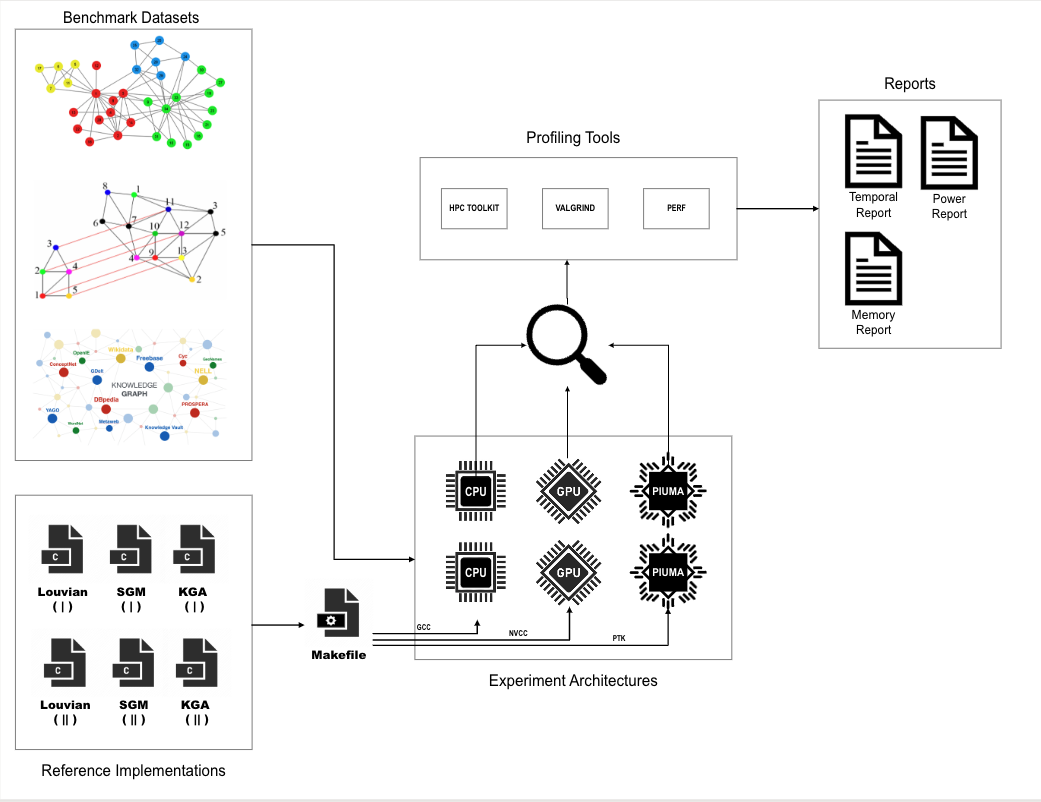
\includegraphics[width=\columnwidth]{Papers/ARLIS_MPR_MN/Figures/high_level_overview.png}
            \caption{A high level schematic diagram of the project framework, tasks, and deliverables}
            \label{fig:highLevelOverview}
        \end{figure*}

    
    \section{Dataset Creation Tool}\label{section:datasetCreation}
        To conduct our initial benchmark testing, we recognized the need to provide a tool for generating graphs with a specific number of nodes and edges. We developed a dataset generator program which takes three command-line arguments: the number of nodes in the graph, the number of edges, and a random seed. The dataset generator creates random datasets in a reproducible manner, serving as a basic introductory collection of test sets, yet its use will be absolved once we develop a more robust benchmarking suite. Future improvements to this creation tool involve curating custom datasets that reflect the structure and properties of real-world social networks, considering metrics such as cluster coefficient, assortativity, and distribution fit. 
        Additionally, scale-free graphs have been identified as a valuable model for capturing characteristics of complex networks observed in domains such as social, biological, and technical networks \cite{Newman2003}. The pioneering work \cite{Barabasi1999} introduced the concept of scale-free networks, where the degree distribution follows a power-law distribution. Scale-free graphs adopt a preferential attachment mechanism \cite{Rak2020}where a few nodes, known as "hubs", have a significantly higher number of connections compared to the majority of nodes in the network as new nodes have the tendency to connect with already well connected nodes. We acknowledge that relying solely on synthetic graph generation may not fully capture the complex nature of real world networks. To address this limitation, we are also exploring integration of real world data sets, following the example of the GAP Benchmark \cite{Beamer2017}.
        
    \section{Telemetry Tools}\label{section:telemetry}
        Utilizing a standardized set of tools in order to evaluate algorithmic performance on multiple architectures is critical in attaining precise benchmarking results. As mentioned in Section \ref{section:metrics}, we need to identify a standard to count the traversed edges per second, measure total execution time, measure spatial locality, measure temporal locality and measure power consumption given each of these other views. Additionally, for parallel implementations, we need to measure network latency as data is passed back and forth between the workers. We are experimenting with basic utilities such as PERF \footnote{\href{https://perf.wiki.kernel.org/index.php/Main_Page}{https://perf.wiki.kernel.org/index.php/Main_Page}}, OPROFILE \footnote{\href{https://oprofile.sourceforge.io/about/}{https://oprofile.sourceforge.io/about/}}, and GNU PROF \footnote{\href{http://web.archive.org/web/20141129061523/http://www.cs.utah.edu/dept/old/texinfo/as/gprof.html#SEC2}{http://web.archive.org/web/20141129061523/http://www.cs.utah.edu/dept/old/texinfo/as/gprof.html#SEC2}}as well as more robust application systems such as HPC Toolkit \footnote{\href{http://hpctoolkit.org/}{http://hpctoolkit.org/}}, VALGRIND \footnote{\href{https://valgrind.org/docs/manual/quick-start.html}{https://valgrind.org/docs/manual/quick-start.html}}, and Intel VTUNE Profiler\footnote{\href{https://www.intel.com/content/www/us/en/developer/tools/oneapi/vtune-profiler.html#gs.11c0nr}{https://www.intel.com/content/www/us/en/developer/tools/oneapi/vtune-profiler.html#gs.11c0nr}}. The tools outlined above will enable us to capture the necessary benchmarking information, relying on an AWS EC2 instance to run the telemetry on an Ubuntu system. We are also simultaneously considering adopting a CENTOS system to run on an EC2 Metal instance as it appears to be a more suitable environment for running the PiUMA simulator.
       
    \section{Interfacing with Clients and Customers}\label{section:stakeholders}  
        \textbf{Agency:} DARPA\\  
        \textbf{POC:} Johnny Marsh \\
        \textbf{Date:} 7/12/23 \\
        \textbf{Purpose:} Communicate Progress on Tasks \\
        \textbf{High-level Takeaway(s):} N/A \\ 
        %\textit{[Repeat per engagement]} 

    \section{Next Steps}\label{section:nextSteps}
        The project has been moving slightly slower than anticipated in regards to the implementation and evaluation of algorithms, yet making steady progress in setting up a robust experimental framework.
        An open source implementation of the Sequentual Louvain algorithm has been successfully implemented on a CPU architecture. 
        Telemetry capabilities have been integrated to measure time, memory and power, providing valuable insights into algorithm performance. 
        Additionally, the NVIDIA CUDA GPU architecture has been successfully configured remotely on the cloud, enabling us to run algorithms across both CPU and GPU architectures. 
        Finally, a dataset creation tool has been developed to produce graphs of various sizes. 
        Current setbacks include having delayed access to a Linux system to run the PiUMA SDV and benchmarking tools. 
        Future anticipated challenges include identifying efficient implementations of subgraph matching and knowledge graph algorithms. 
        Looking ahead, the project will focus on implementing and evaluating subgraph matching and knowledge graph algorithms. 
        The telemetry capabilities will be expanded to include additional metrics and dimensions for a more comprehensive analysis. 
        The dataset creation process will continue to evolve by incorporating more realistic and diverse data formats while also considering scale free graphs and real-world datasets. 
        By advancing these aspects, the project is on track to deliver benchmarking results of atleast two out of three graph processing algorithms on both CPU and GPU architectures. 
        Setting up the PiUMA framework continues to remain a task in progress, but is targeted for completion by the end of the month.
        Overall progress is slow due to the necessity of setting up an extensive testing framework, yet is on track to pick up pace as familiarity with tools/algorithms increases, ultimately contributing to HIVE's vision of increasing processing of streaming graphs at significantly higher speeds. 
        
    \section{References}
        \printbibliography[heading=none]

    \section{Acronyms}
        \small{
        \textbf{ARLIS} Applied Research Laboratory for Intelligence and Security.\\ 
        \textbf{BFS} Breadth First Search \\
        \textbf{CPU} Central Processing Unit \\
        \textbf{DARPA} Defense Advanced Research Projects Agency \\ 
        \textbf{GPU} Graphics Processing Unit \\
        \textbf{HIVE} Hierarchical Identify Verify Exploit \\
        \textbf{KGA} Knowledge Graph Analytics \\
        \textbf{PIUMA} Programmable Integrated Unified Memory Architecture \\ 
        \textbf{SGM} Sub Graph Matching \\
        }
    }
    \end{multicols}
    \newpage
\end{document}
